\section{Surface Parameterization Methods}


This package provides a second \ccc{parameterize()} entry point
where the user can specify a parameterization method:

\ccFunction{Parameterizer_traits_3<ParameterizationMesh_3>::Error_code parameterize (ParameterizationMesh_3 * mesh, ParameterizerTraits_3 parameterizer);}
{ Compute a ont-to-one mapping from a 3D triangle surface 'mesh' to a
simple 2D domain. The mapping is piecewise linear on the triangle
mesh. The result is a pair (u,v) of parameter coordinates for each
vertex of the input mesh.  One-to-one mapping may be guaranteed or
not, depending on the chosen ParametizerTraits\_3 algorithm.
Preconditions:\begin{itemize}
\item 'mesh' must be a surface with one connected component.\item
'mesh' must be a triangle mesh.\item the mesh boundary must be mapped onto a convex polygon (for fixed border parameterizations).\end{itemize}
}


This \cgal\ package implements some of the state-of-the-art surface
parameterization methods which can be used as
\ccc{ParameterizerTraits_3} parameter.

This package also provides common parameterization methods for
boundaries which are used as traits classes modifying the behavior of
the \ccc{ParameterizerTraits_3} methods.


\subsection{Fixed Border Surface Parameterizations}

Fixed Border Surface Parameterizations need a
set of constraints: two u,v coordinates for each vertex along the border.

\subsubsection{Tutte Barycentric Mapping}

\ccc{CGAL::Barycentric_mapping_parameterizer_3}  \\

The Barycentric Mapping parameterization method has been introduced by
Tutte~\cite{cgal:fh-survey-05}. In parameter space, each vertex is
placed at the barycenter of its neighbors. This amounts to solve one
sparse linear solver for each set of parameter coordinates, with a
\#vertices x \#vertices sparse matrix. A coefficient $(i,j)$ of the
matrix is set to 1 for an edge linking the vertex $i$ to the vertex
$j$, to the degree of . It is

Coefficients are quickly computed (non diagonal coefficients
are either 1 or 0). The matrix (the same for both systems) is
symmetric definite positive, thus can be efficiently solved.

Tutte Barycentric Mapping is the fastest method, but results are not visually pretty.
Usage is recommended when the caller wishes any one-to-one mapping and is
interested by speed.

% Include uniform.png/eps figure with title =
% "Tutte Barycentric Mapping (the red line emphasizes the cutting path)"
\begin{figure}[bht]
    \begin{center}
        % Image
        \begin{ccTexOnly}
            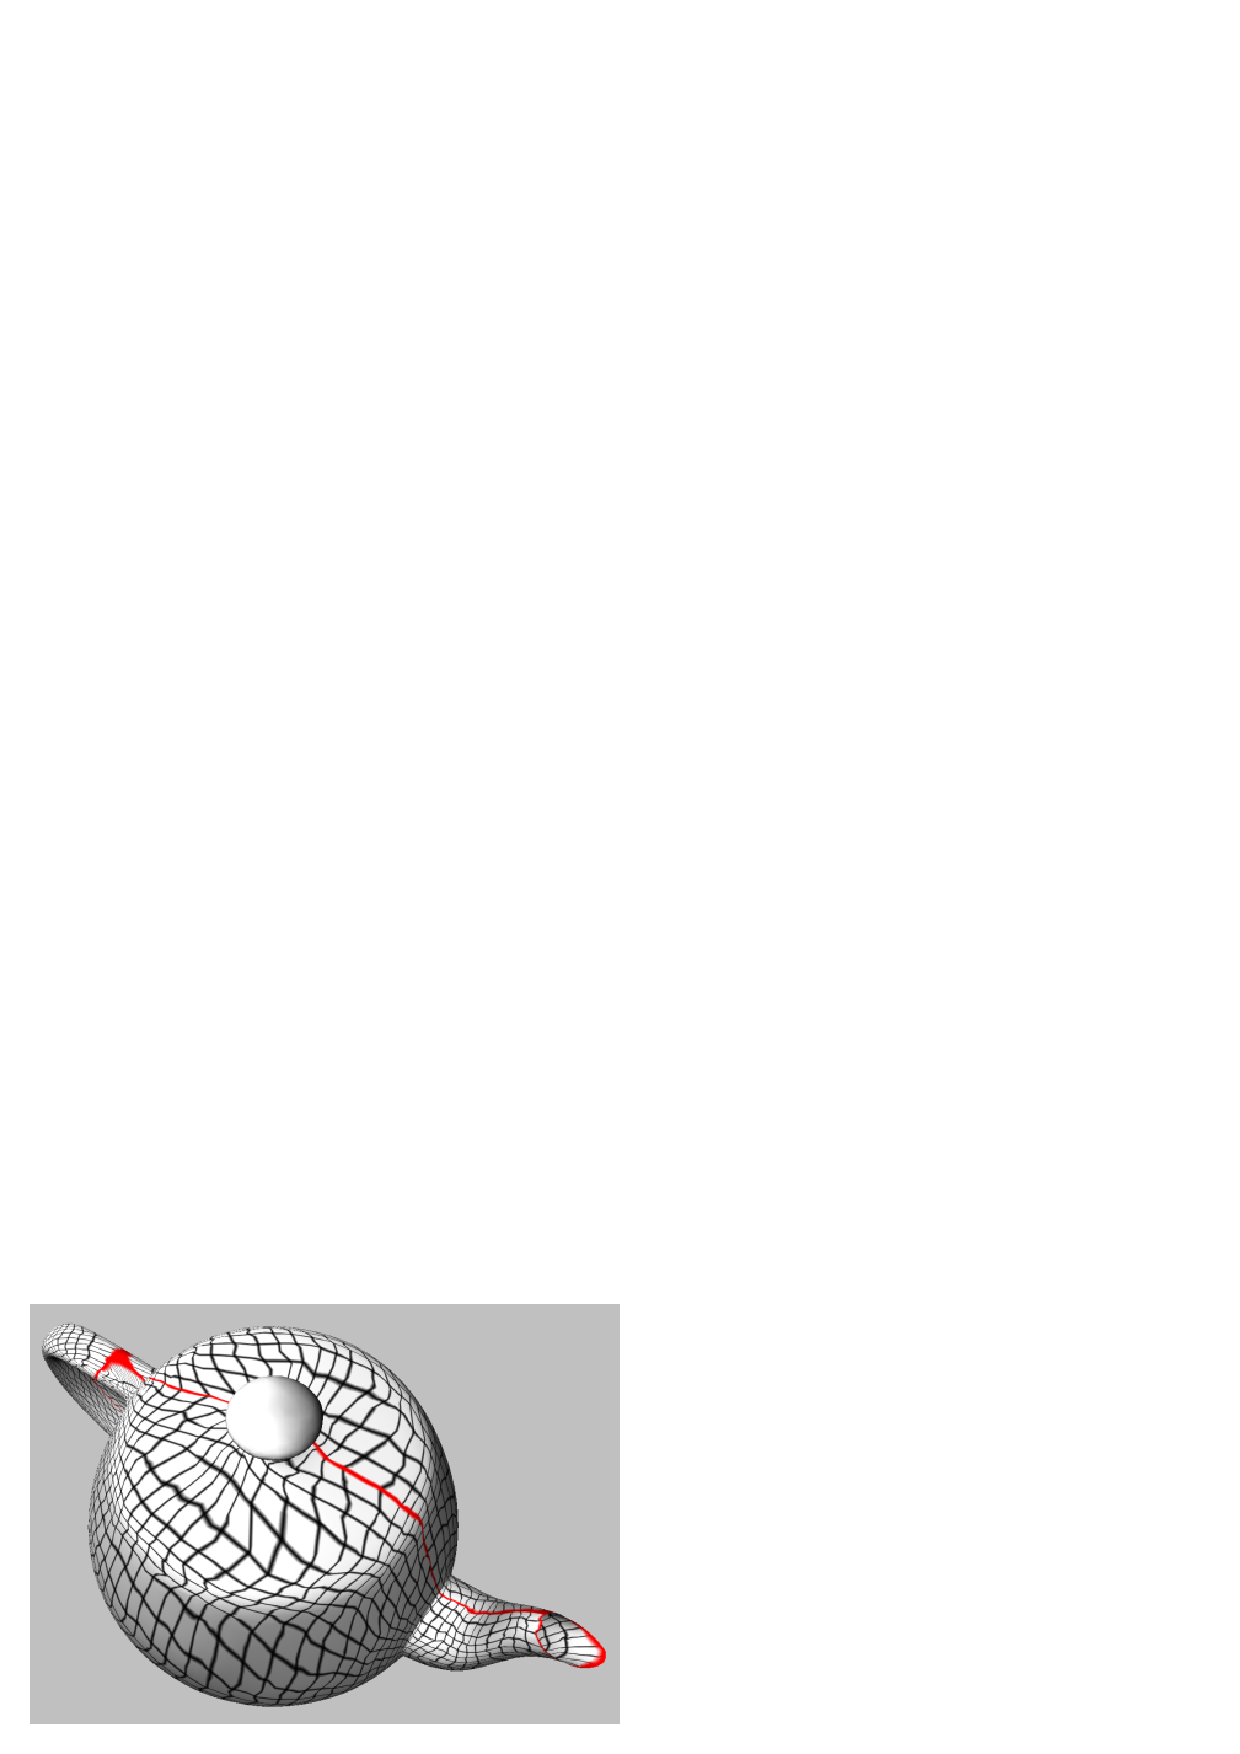
\includegraphics{Parameterization/uniform} % omit suffix to support PS and PDF
        \end{ccTexOnly}
        \begin{ccHtmlOnly}
            <img border=0 src="./uniform.png" align=center>
        \end{ccHtmlOnly}
        \label{parameterization-fig-uniform}

        % Title
        \caption{Tutte Barycentric Mapping (the red line emphasizes the cutting path)}
    \end{center}
\end{figure}


\subsubsection{Discrete Conformal Map}

\ccc{CGAL::Discrete_conformal_map_parameterizer_3}  \\

Discrete Conformal Map parameterization, by Eck et a. or Pinkall and Polthier
\cite{cgal:fh-survey-05}, is one of the earliest conformal methods. It attempts
to lower angle deformation by minimizing the Dirichlet energy.

One-to-one mapping is conditionally guaranteed if all weights
of the linear system are positive and border is convex.

This method solves two \#vertices x \#vertices sparse linear systems. The matrix
(the same for both systems) is symmetric definite positive, thus can be
efficiently solved.

When one-to-one mapping is achieved, Discrete Conformal Map gives aesthetic results:

% Include conformal.png/eps figure with title = "Discrete Conformal Map"
\begin{figure}[bht]
    \begin{center}
        % Image
        \begin{ccTexOnly}
            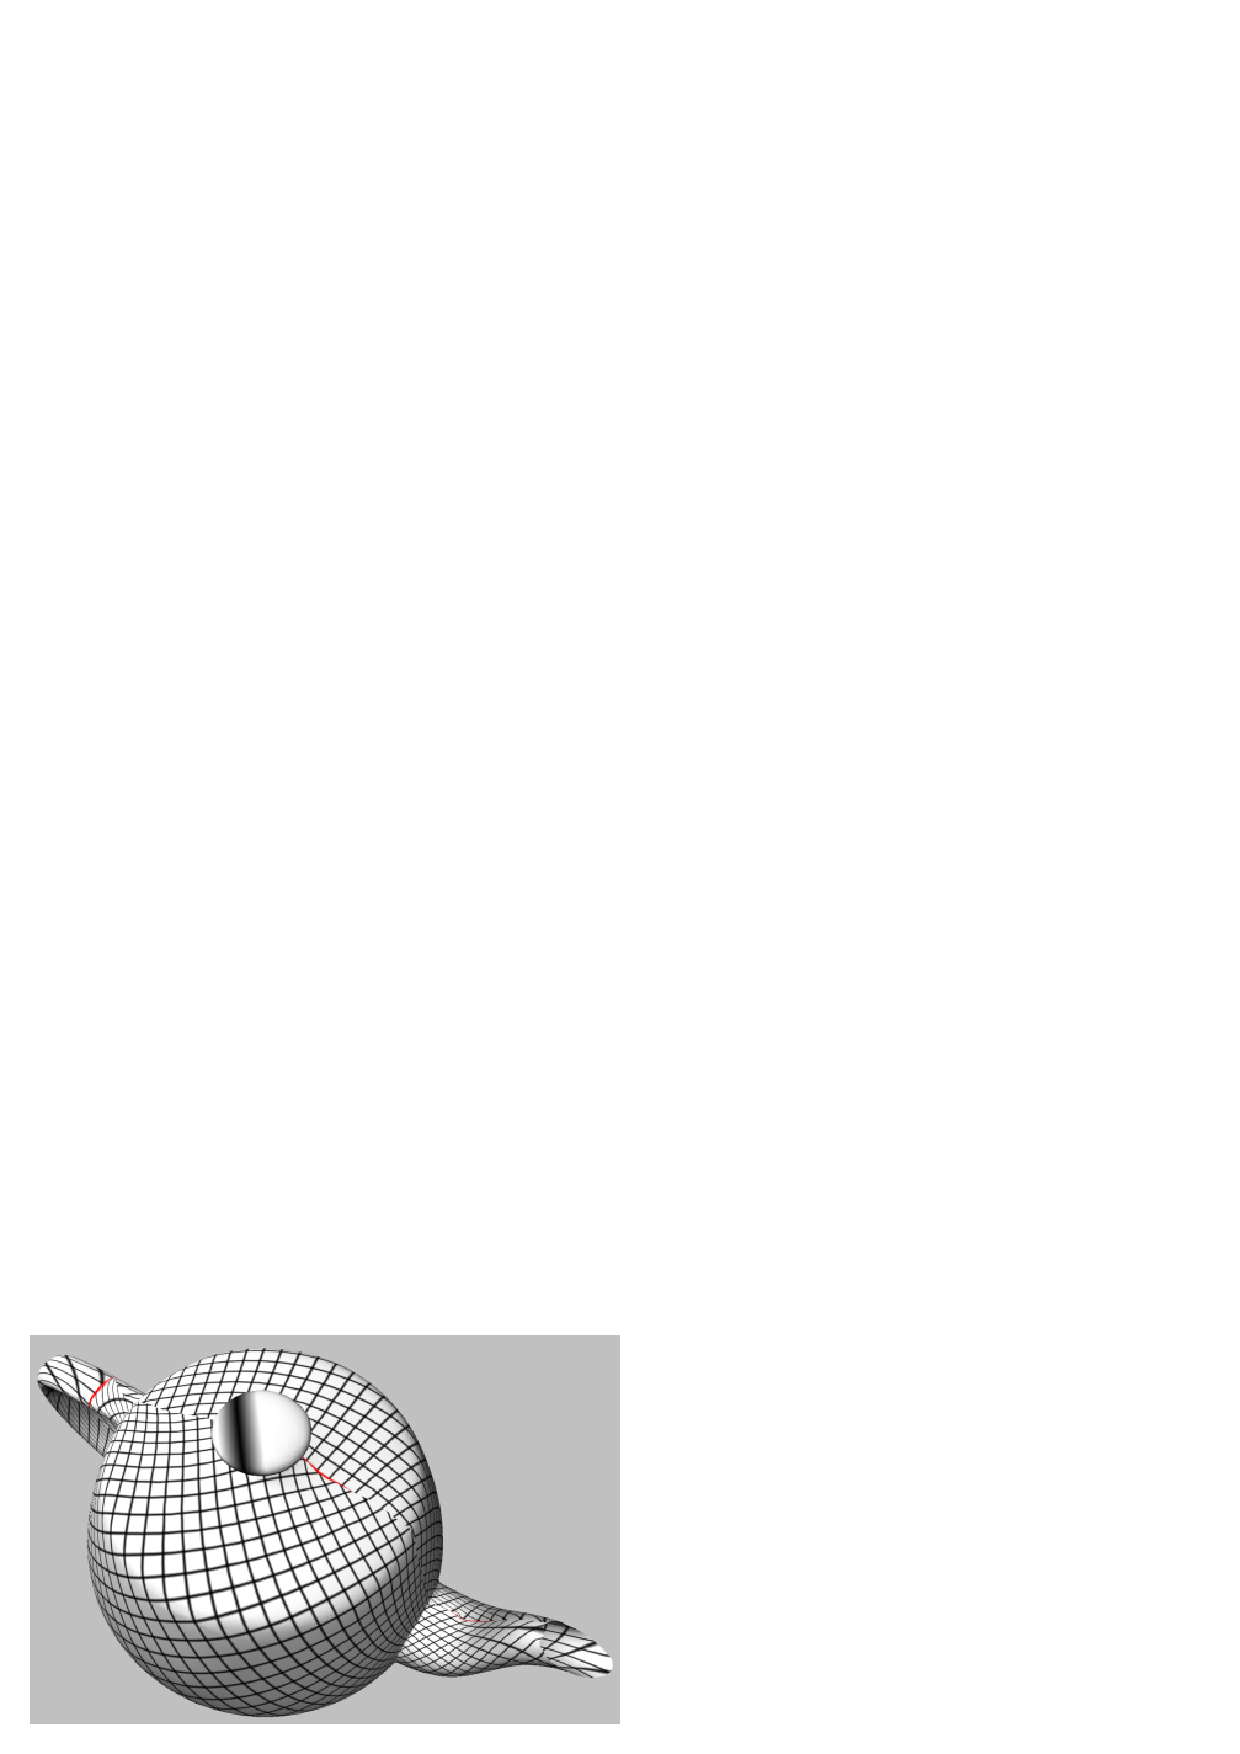
\includegraphics{Parameterization/conformal} % omit suffix to support PS and PDF
        \end{ccTexOnly}
        \begin{ccHtmlOnly}
            <img border=0 src="./conformal.png" align=center>
        \end{ccHtmlOnly}
        \label{parameterization-fig-conformal}

        % Title
        \caption{Discrete Conformal Map}
    \end{center}
\end{figure}


\subsubsection{Floater Mean Value Coordinates}

\ccc{CGAL::Mean_value_coordinates_parameterizer_3}  \\

Mean Value Coordinates parameterization, by Floater \cite{cgal:f-mvc-03},
is a conformal method that does not minimize an energy. Visual results
are close to, but a little less pretty than Discrete Conformal Map.

In the other hand, one-to-one mapping is guaranteed.

This method solves two \#vertices x \#vertices sparse linear systems. The matrix
(the same for both systems) is asymmetric.

% Include floater.png/eps figure with title = "Floater Mean Value Coordinates"
\begin{figure}[bht]
    \begin{center}
        % Image
        \begin{ccTexOnly}
            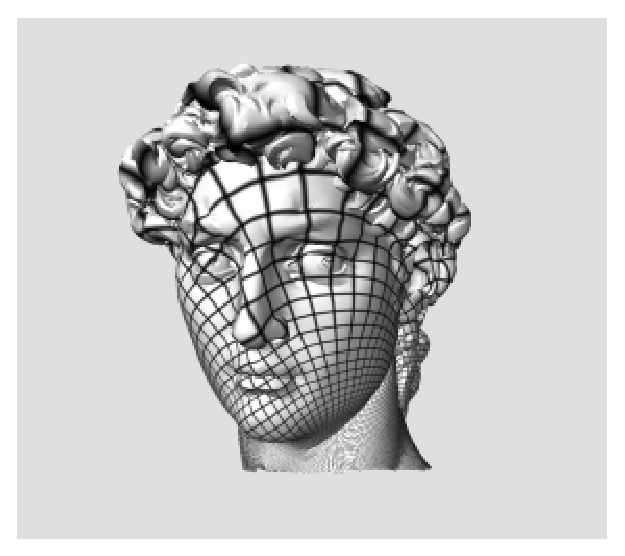
\includegraphics{Parameterization/floater} % omit suffix to support PS and PDF
        \end{ccTexOnly}
        \begin{ccHtmlOnly}
            <img border=0 src="./floater.png" align=center>
        \end{ccHtmlOnly}
        \label{parameterization-fig-floater}

        % Title
        \caption{Floater Mean Value Coordinates}
    \end{center}
\end{figure}


\subsubsection{Discrete Authalic parameterization}

\ccc{CGAL::Discrete_authalic_parameterizer_3}  \\

Discrete Authalic parameterization, by Desbrun, Meyer and Alliez
\cite{cgal:dma-ipsm-02}, is the only authalic method provided
by this package. It is a weak area-preserving method:
it computes a compromise between area and angle preserving by
minimizing a {\em chi energy}.

One-to-one mapping is conditionally guaranteed if all weights
of the linear system are positive and border is convex.

This method solves two \#vertices x \#vertices sparse linear systems. The matrix
(the same for both systems) is asymmetric.

% Include authalic.png/eps figure with title = "Discrete Authalic Parameterization"
\begin{figure}[bht]
    \begin{center}
        % Image
        \begin{ccTexOnly}
            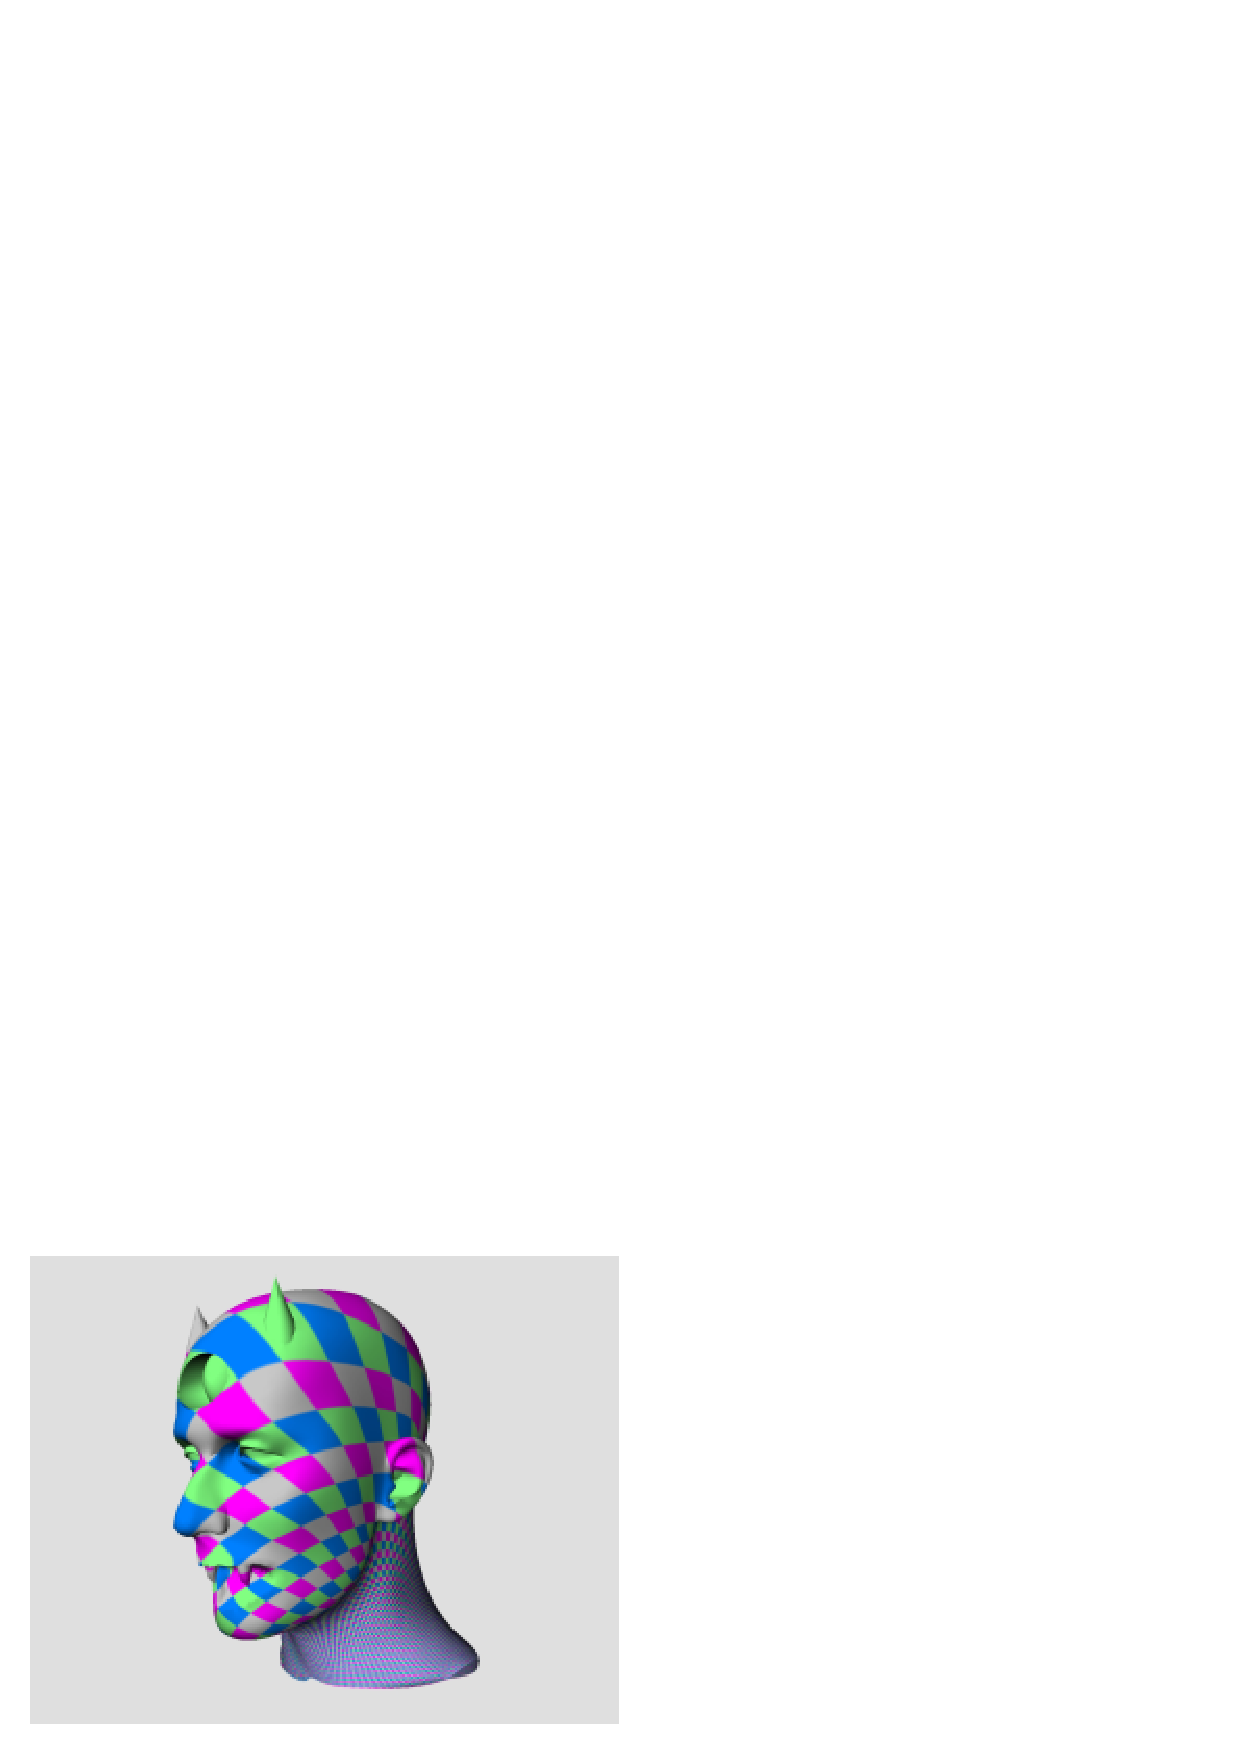
\includegraphics{Parameterization/authalic} % omit suffix to support PS and PDF
        \end{ccTexOnly}
        \begin{ccHtmlOnly}
            <img border=0 src="./authalic.png" align=center>
        \end{ccHtmlOnly}
        \label{parameterization-fig-authalic}

        % Title
        \caption{Discrete Authalic Parameterization}
    \end{center}
\end{figure}


\subsubsection{Associated Border Parameterization}

Border Parameterizations for Fixed Border Surface Parameterizations
are a family of methods to define a
set of constraints: two u,v coordinates for each vertex along the border.

\begin{itemize}

\item The user can select a border parameterization among
two common methods: uniform or arc-length parameterization.
Arc-length border parameterization is the default as it minimizes distortion.
Uniform border parameterization is recommended when the caller wishes
any one-to-one mapping and is interested by speed.

\item One convex shape specified by:

    \begin{itemize}

    \item one shape among a set of standard ones (circle, square).
    Circular border parameterization is the default as it minimizes distortion.
    Square border parameterization is interesting for texture mapping.

    \item a convex polygon.

    (not yet implemented)

    \end{itemize}

\end{itemize}

\ccc{CGAL::Circular_border_arc_length_parameterizer_3}  \\
\ccc{CGAL::Circular_border_uniform_parameterizer_3}  \\
\ccc{CGAL::Square_border_arc_length_parameterizer_3}  \\
\ccc{CGAL::Square_border_uniform_parameterizer_3}  \\


\subsection{Free Border Surface Parameterizations}

\subsubsection{Least Squares Conformal Maps}

\ccc{CGAL::LSCM_parameterizer_3}  \\

Least Squares Conformal Maps parameterization, by Levy et al.
\cite{cgal:lprm-lscm-02}, is a conformal method with a free
border (only two border vertices must be fixed to have a unique solution).

One-to-one mapping is conditionally guaranteed if all weights
of the linear system are positive.

This method solves a (2 * \#triangles) x \#vertices sparse linear system
in the least squares sense.

% Include LSCM.png/eps figure with title = "Least Squares Conformal Maps"
\begin{figure}[bht]
    \begin{center}
        % Image
        \begin{ccTexOnly}
            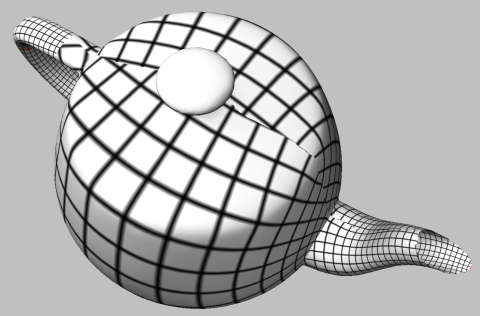
\includegraphics{Parameterization/LSCM} % omit suffix to support PS and PDF
        \end{ccTexOnly}
        \begin{ccHtmlOnly}
            <img border=0 src="./LSCM.png" align=center>
        \end{ccHtmlOnly}
        \label{parameterization-fig-LSCM}

        % Title
        \caption{Least Squares Conformal Maps}
    \end{center}
\end{figure}


\subsubsection{Natural Conformal Map}

(not yet implemented)

Natural Conformal Map parameterization, by Desbrun, Meyer and Alliez
\cite{cgal:dma-ipsm-02}, achieves the same result as
Least Squares Conformal Maps by an independent
way (extending the Discrete Conformal Map method). Again,
two border vertices must be fixed to have a unique solution.

One-to-one mapping is conditionally guaranteed if all weights
of the linear system are positive.

This method solves a (2 * \#vertices) x \#vertices sparse linear system.
The matrix is symmetric definite positive, thus can be
efficiently solved. The conditionning is less good as Least Squares Conformal Maps.


\subsubsection{Associated Border Parameterization}

\ccc{CGAL::Two_vertices_parameterizer_3}  \\

The associated Border Parameterization method defines only two constraints
(the pinned vertices). They have to be on the specified border.


\subsection{Discrete Authalic Parameterization Example}

The code below applies a Discrete Authalic parameterization to a \ccc{Polyhedron_3} mesh:

\begin{ccExampleCode}

// CGAL kernel
typedef CGAL::Cartesian<double>                         Kernel;

// Mesh true type and parameterization adaptors
typedef CGAL::Polyhedron_3<Kernel>                      Polyhedron;
typedef CGAL::Parameterization_polyhedron_adaptor_3<Polyhedron>
                                                        Parameterization_polyhedron_adaptor;

// Discrete Authalic Parameterization
typedef CGAL::Discrete_authalic_parameterizer_3<Parameterization_polyhedron_adaptor>
                                                        Parameterizer;

int main(int argc,char * argv[])
{
    Polyhedron mesh;
    ...

    // The parameterization package needs an adaptor to handle Polyhedron_3 meshes
    // The mesh must be a topological disk
    Parameterization_polyhedron_adaptor mesh_adaptor(&mesh);

    // Discrete Authalic Parameterization
    Parameterizer::Error_code err = CGAL::parameterize(&mesh_adaptor, Parameterizer());
    ...
}

\end{ccExampleCode}

See the complete code in \ccc{Authalic_parameterization.C} example.


\subsection{Square Border Arc Length Parameterization Example}

The code below applies a Floater Mean Value Coordinates parameterization
with a Square Border Arc Length parameterization:

\begin{ccExampleCode}

// CGAL kernel
typedef CGAL::Cartesian<double>                         Kernel;

// Mesh true type and parameterization adaptors
typedef CGAL::Polyhedron_3<Kernel>                      Polyhedron;
typedef CGAL::Parameterization_polyhedron_adaptor_3<Polyhedron>
                                                        Parameterization_polyhedron_adaptor;

// Square border parameterizer
typedef CGAL::Square_border_arc_length_parameterizer_3<Parameterization_polyhedron_adaptor>
                                                        Border_parameterizer;

// Floater Mean Value Coordinates parameterizer with square border
typedef CGAL::Mean_value_coordinates_parameterizer_3<Parameterization_polyhedron_adaptor,
                                                     Border_parameterizer>
                                                        Parameterizer;

int main(int argc,char * argv[])
{
    Polyhedron mesh;
    ...

    // The parameterization package needs an adaptor to handle Polyhedron_3 meshes
    // The mesh must be a topological disk
    Parameterization_polyhedron_adaptor mesh_adaptor(&mesh);

    // Floater Mean Value Coordinates parameterization
    // with a Square Border Arc Length Parameterization
    Parameterizer::Error_code err = CGAL::parameterize(&mesh_adaptor, Parameterizer());
    ...
}

\end{ccExampleCode}

See the complete code in \ccc{Square_border_parameterization.C} example.
